\documentclass[aspectratio=169,t,xcolor=table]{beamer}
\usepackage[utf8]{inputenc}%utf8

\usepackage{booktabs} 
\usepackage{subcaption}
\usepackage{ragged2e}%Texto justificado 02/11/2022
\usepackage[alf,abnt-repeat-title-omit=yes,abnt-emphasize=bf,abnt-etal-list=0]{abntex2cite}%abntex 02/11/2022
\usepackage[english,brazil]{babel}%08/11/2022
%-----------------------------------------------------------
\def\autorc{Wagner O. de Araujo}
\def\autora{Josiel P. C. Silva}
\def\autorb{ Matheus L. de Andrade}
\def\professor{Prof. Arlindo Rodrigues Galvão Filho, D.Sc.}
\def\titulo{Classificação Interpretável de Questões Acadêmicas com Redes Neurais: uma Abordagem Baseada em Camadas de Atenção}
\def\curso{Instituto de Informática}
\def\disciplina{Processamento de Linguagem Natural}

\usetheme{Ufg}

%-------------------------------------theorems--------------
\newtheorem{conj}{Conjetura}
\newtheorem{defi}{Definição}
\newtheorem{teo}{Teorema}
\newtheorem{lema}{Lema}
\newtheorem{prop}{Proposição}
\newtheorem{cor}{Corolário}
\newtheorem{ex}{Exemplo}
\newtheorem{exer}{Exercício}

\setbeamertemplate{theorems}[numbered]
\setbeamertemplate{caption}[numbered]

%-------------------------------------------------------------%
%----------------------- Primary Definitions -----------------%

% This command set the default Color, is also possible to choose a custom color
\setPrimaryColor{DarkGreen} %LightGreen%UFGBlue

% First one is logo in title slide (we recommend use a horizontal image), and second one is the logo used in the remaining slides (we recommend use a square image)
\setLogos{lib/logos/infw.png}{lib/logos/infw2.png} 


% -------------------------------------- Title Slide Information
\begin{document}
\title[Inf UFG]{\titulo}
\subtitle{}

\author{\autora\inst{1} \and \autorb\inst{1} \and \autorc\inst{1}
}

\institute[UFG] % (optional)
{
  \inst{1}%
  %Escola de Engenharia Civil e Ambiental\\
	%Programa de Pós-graduação em Geotecnia, Estruturas e Construção Civil\\
  Universidade Federal de Goiás\\
	Campus: Samambaia\\
	\curso\\
	\disciplina\\
	\professor
 % \and
 % \inst{2}%
 % Instituto de Informática\\
 % Federal University of Goiás
}
\date{2024.2}
%-----------------------The next statement creates the title page.
\frame[noframenumbering]{\titlepage}


%------------------------------------------------Slide 1
\setLayout{vertical} % This command define the layout. 'vertical' can be replace with 'horizontal', 'blank, 'mainpoint', 'titlepage'

\begin{frame}
    \frametitle{Sumário}
    \tableofcontents
\end{frame}
%-------------------------------------------------------


%---------------------------------------------------------Slide 2
\section{Introdução}

\subsection{Box}

\setLayout{vertical}
\begin{frame}{Introdução}

    \footnotesize
    
    \begin{ex}
        Em uma versão da linguagem BASIC, o nome de uma variável é uma sequência de um ou dois caracteres alfanuméricos, em que letras maiúsculas e minúsculas não são distinguidas. Além disso, um nome de variável deve começar com uma letra e deve ser diferente das cinco sequências de dois caracteres reservadas para o uso de comandos. Quantos nomes diferentes de variáveis são possíveis nesta versão do BASIC?
    \end{ex}
    
    \begin{block}{Solução}
        Pela regra da soma, $V=V_1+V_2$. Como as variáveis só podem começar com letras, temos que $V_1=26$. Pela regra do produto, há $26\cdot 36=936$ sequências de tamanho $2$ que comecem com uma letra e terminam com um carácter alfanumérico. Porém, não se deve usar $5$ variáveis reservadas. Assim, $V_2=26\cdot 36-5=931$. Logo, há $V=V_1+V_2 = 26+931=957$ nomes diferentes para variáveis nesta versão do BASIC.
    \end{block}

\end{frame}
%---------------------------------------------------------
\def\artigo{Título do artigo}

\setLayout{UFGBlue}
\begin{frame}
	\frametitle{\artigo}
	\begin{columns}
		\begin{column}{.52\textwidth}%52
\begin{itemize}
 \item \justifying{Este método de teste abrange o teste de campo com palhetas em solos macios, saturados e coesivos. O conhecimento da natureza do solo em que cada teste de palheta deve ser feito é necessário para avaliação da aplicabilidade e interpretação do teste.}
\end{itemize}
\end{column}
		\begin{column}{.52\textwidth}%45
\begin{figure}
%[width=0.8 \textwidth]-[width=5.25cm,height=7.4cm]
%[width=4.79cm,height=6.20cm]
\pgfdeclareimage[width=0.65 \textwidth]{astm}{figs/NBR10905_V2}\label{fig:astm}
		\pgfuseimage{astm}
%\caption{Coeficiente de determinação.}
\end{figure}
		\end{column}
	\end{columns}
\end{frame}


%--------------------------------------------------------- Slide 3
\subsection{Table}
\setLayout{vertical}
\begin{frame}{Example on using table}

    \begin{table}[]
        \centering
        \caption{\label{tab:1}Countries and their codes.}
        
        \renewcommand{\arraystretch}{1.5}
        \setlength{\tabcolsep}{10pt}
        
        {\rowcolors{2}{}{LightGray!20}
            \begin{tabular}{ p{3cm}p{3cm}p{3cm}  }
                \toprule 
                \textbf{Country Name} & \textbf{Code 2} & \textbf{Code 3} \\
                \midrule
                Afghanistan & AF &AFG \\
                Aland Islands & AX   & ALA \\
                Albania &AL & ALB \\
                Algeria    &DZ & DZA \\
                \bottomrule
								\multicolumn{3}{l}{Fonte: O Autor} \\ 
            \end{tabular}
        }
    \end{table}
    
\end{frame}
%---------------------------------------------------------

\subsection{Image}

%--------------------------------------------------------- Slide 4
\begin{frame}{Example on using image}

    \begin{figure}
        \centering
				\caption{Template's Layouts.}
        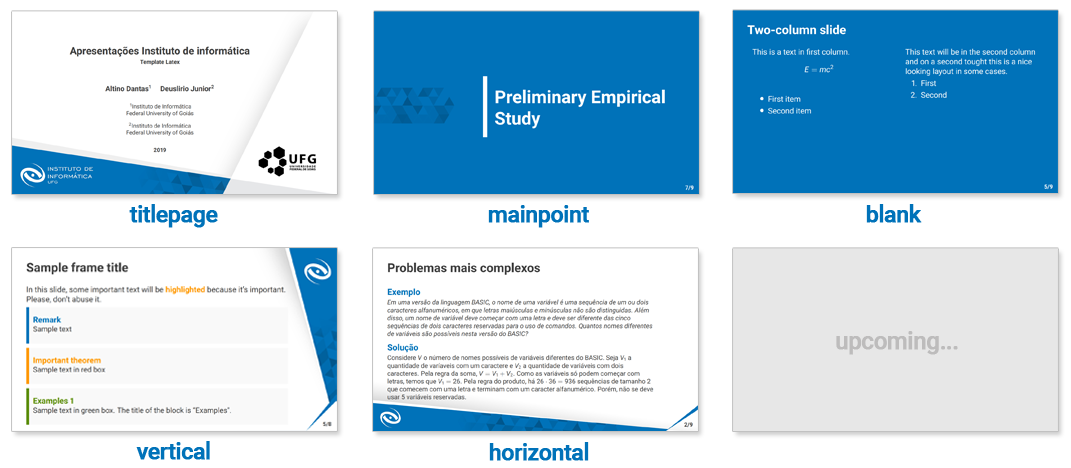
\includegraphics[width=.9\textwidth]{readme/layouts.png}
        %\caption{Template's Layouts.}
        \label{fig:layouts}
    \end{figure}
    
\end{frame}
%---------------------------------------------------------

\begin{frame}
\frametitle{Desenvolvimento}

\begin{block}{Titulo do bloco}
\begin{description}
	\item<1->[a)] alínea a;
	\item<2->[b)] alínea b;
	\item<3->[c)] alínea c;
	\item<4->[d)] alínea d.
\end{description}
\end{block}
	
\end{frame}

\begin{frame}
\frametitle{Título do slide 2}
\begin{table}[]
\centering
\caption{Matriz $4\times 4$.}
\begin{tabular}{p{0.5cm}|p{0.5cm}|p{0.5cm}|p{0.5cm}}
\hline
a11 & a12 & a13 & a14 \\ 
\hline
a21 & a22 & a23 & a24 \\ 
\hline
a31 & a32 & a33 & a34 \\ 
\hline
a41 & a42 & a43 & a44 \\ 
\hline
\multicolumn{4}{l}{Fonte: O Autor} \\ 
\end{tabular}
%\begin{center}
%Fonte: O Autor
%\end{center}
\end{table}

\end{frame}

%--------------------------------------------------------- Slide 5
\section{Desenvolvimento}

\setLayout{blank}%Exemplo de slide: titlepage,mainpoint,blank,vertical,horizontal
\setBGColor{UFGBlue}%UFGBlue,DarkOrange  %Example of changing background color 

\begin{frame}{Clean layout and two-column text}
    
    \begin{columns}
        \column{0.5\textwidth}
        This is a text in first column.
        $$E=mc^2$$
        $$ 1 + 2 + \cdots + k =  \frac{k \cdot (k + 1)}{2}.$$
        \begin{itemize}
        \item First item;
        \item Second item.
        \end{itemize}
        
        \column{0.5\textwidth}
        This text will be in the second column
        and on a second tought this is a nice looking
        layout in some cases.
        
        \begin{enumerate}
            \item First
            \item Second
        \end{enumerate}
    \end{columns}
    
\end{frame}
%---------------------------------------------------------


%---------------------------------------------------------Slide 6
%Highlighting text
\setLayout{vertical}
\begin{frame}{Sample frame title}
    
    In this slide, some important text will be
    \alert{highlighted} because it's important. Please, don't abuse it.
    
    \begin{block}{Remark}
        Sample text
    \end{block}
    
    \begin{alertblock}{Important theorem}
        Sample text in \colorbox[rgb]{1,0,0}{alert box}
    \end{alertblock}
    
    \begin{examples}
        Sample text in green box. The title of the block is ``Examples".
    \end{examples}
    
\end{frame}
%---------------------------------------------------------


%---------------------------------------------------------Slide 7
\section{Conclusão}

\setLayout{mainpoint}%Tipo do slide
\setBGColor{UFGBlue}%Cor do slide DarkPurple
\begin{frame}
    \frametitle{Conclusão}
\end{frame}
%-------------------------------------------------------


%---------------------------------------------------------Slide 8

\setLayout{horizontal}
\begin{frame}
    \frametitle{Sample frame title}
    This is a text in second frame. For the sake of showing an example.
    
    \begin{itemize}
        \item<1-> Text visible on slide 1
        \item<2-> Text visible on slide 2
        \begin{itemize}
            \item text subitem
        \end{itemize}
        \item<3> Text visible on slides 3
        \item<4-> Text visible on slide 4
    \end{itemize}
\end{frame}
%---------------------------------------------------------

%---------------------------------------------------------
\setLayout{vertical}
\begin{frame}
%\frametitle{Introdução}
   \frametitle{Ensaios \textit{in situ} (métodos semidiretos)}
\justifying{ O ensaio de palheta foi originalmente utilizado em 1919 (FLODIN; BROMS,1981) na Suécia, durante a construção da ponte Lidingö, em Estocolmo, que ocorreu no período de 1917 a 1926 (NORDENDAHL, 1928; COLLET, 1978).
Naquela ocasião foi utilizada uma palheta desenvolvida por Jonh Olsson, construída por \textcolor[rgb]{0,0,1}{C. Forssell} foi apresentada no 3º Congresso Internacional de Mecânica Aplicada em Estocolmo 1930. Jonh Olsson, foi responsável pelas investigações
geotécnicas na obra, sendo este o desafio de estimar os coeficientes horizontais de reação do solo, necessários para a determinação dos comprimentos dos elementos estruturais de fundação a serem implantados numa região com profundidades acima de 40 metros de solos moles (SOUZA, 2014).
Chegou ao Brasil em 1949, pelo Instituto de Pesquisas Tecnológicas de São Paulo (IPT) sendo normatizado somente em 1989 através da norma MB-3122 e transcrita sem alteração de conteúdo técnico para NBR10905~\cite{NBR10905:1989} \cite{Hopfield_1982,Rumelhart_1986}
}

\end{frame}
%---------------------------------------------------------

%%%%%%%%%%%%%%%%%%%%%%%%%%%%%%%%%%%%%%%%%
%%%%%%%%%%%%Frame 16
%%%%%%%%%%%%%%%%%%%%%%%%%%%%%%%%%%%%%%%%%
\section[Referências]{Referências}
%\subsection[Referências]{Referências}
\setLayout{horizontal}
\begin{frame}[allowframebreaks]
   \frametitle<presentation>{Referências}
	%\begin{thebibliography}{4}
	%\bibliographystyle{abntex2-alf}%abntex2-num ou abntex2-alf
\justifying{
\bibliography{referencias}
%\end{thebibliography}
}
\end{frame}
%---------------------------------------------------------

\section{Agradecimento}
%---------------------------------------------------------Slide 9
\setLayout{blank}%DarkPurple%blank
\begin{frame}
%\frametitle{Titulo}   
    \centering
    \vspace{2cm}
    
    \textbf{\Huge Thanks}%Titulo do slide
    
    \ \\
    
    \textbf{Doubts and Suggestions}
    \ \\
    
    \text{\footnotesize wagner.oliveira@discente.ufg.br}
    
    \vspace{2cm}
    \begin{figure}
        \centering
        \begin{subfigure}{0.2\textwidth}
            \centering
            
\includegraphics[height=1cm]{lib/logos/infw.png}
        \end{subfigure}%
        \qquad 
        \begin{subfigure}{0.2\textwidth}
            \centering
            
\includegraphics[height=1cm]{lib/logos/ufgw.png}
        \end{subfigure}
      
    \end{figure}
    
\end{frame}
%----------------------------------------------------------



%---------------------------------------------------------Slide 10
\setLayout{titlepage}
\setBGColor{DarkGray}
\titlepage
%-------------------------------------

\end{document}
